\documentclass{article}
\usepackage{graphicx}
\usepackage[margin=1.5cm]{geometry}
\usepackage{amsmath}

\begin{document}

\title{Wednesday Reading Assessment: Unit 5, Forces}
\author{Prof. Jordan C. Hanson}

\maketitle

\section{Memory Bank}

\begin{itemize}
\item Force of friction: $f = \mu N$, where $N$ is the normal force, and $\mu$ is the coefficient of friction.
\item Weight force: $w = mg$.
\end{itemize}
\begin{figure}[ht]
\centering
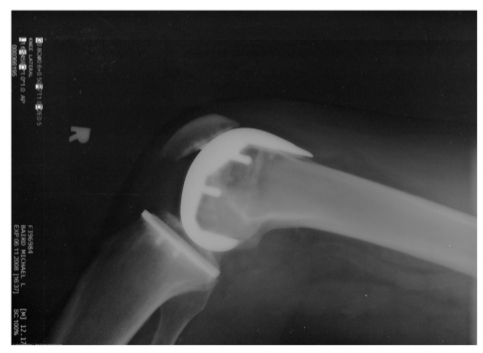
\includegraphics[width=0.3\textwidth]{bone.png}
\caption{\label{fig:bone} An x-ray of the results of a knee-replacement surgery.}
\end{figure}
\section{Chapter 5 - Friction}
\begin{enumerate}
\item The coefficient of friction for a joint comprised of bone and tissue in the human body is about $\mu = 0.015$.  If a person has a mass of 60 kg, what is the (maximum) force of friction on this joint? \\ \vspace{2cm}
\item Suppose as the person gets older, the joint ``wears down'' by providing less and less synovial fluid.  If $\mu$ doubles in value, what is the new force of friction? \\ \vspace{2cm}
\item Suppose the person decides to have a knee replacement surgery (see Fig. \ref{fig:bone}).  The new $\mu$ value is back to 0.015, but the mass of the person has decreased to 55.0 kg for other reasons.  What is the new force of friction in the knee joint?
\end{enumerate}

\end{document}
